\documentclass[10pt]{article}

\usepackage[utf8]{inputenc}
\usepackage[french]{babel}
\usepackage{amsmath}
\usepackage{amsfonts}
\usepackage{amssymb}
\usepackage{graphicx}
\usepackage{parskip}


\begin{document}

\title{IFT2425 - TP3 - Rapport}
\date{Mars 2011}
\author{Vincent Foley-Bourgon (FOLV08078309) \and
  Eric Thivierge (THIE09016601)}

\maketitle

\section{Interpolation}

\subsection{Graphes de l'erreur des polynômes d'interpolation}

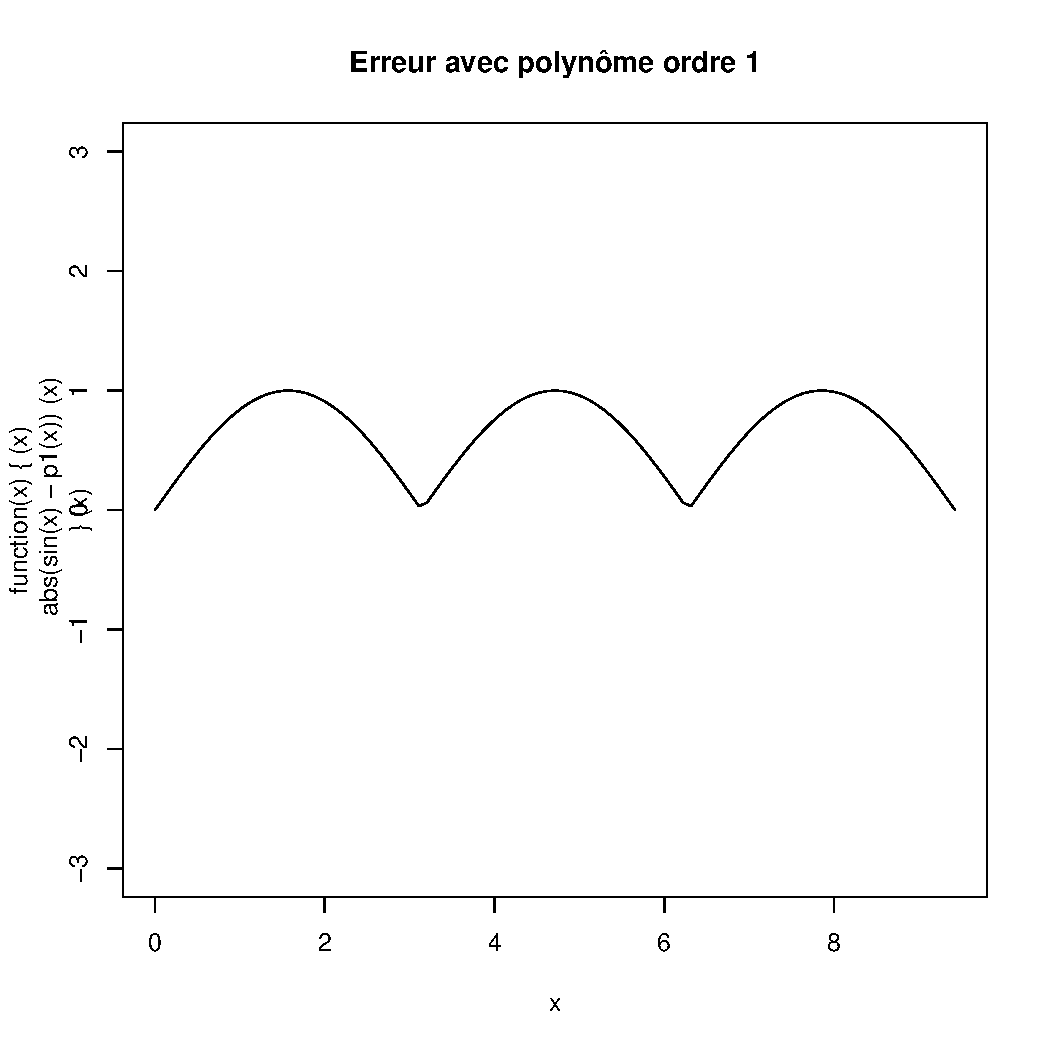
\includegraphics[scale=0.4]{data/p1}
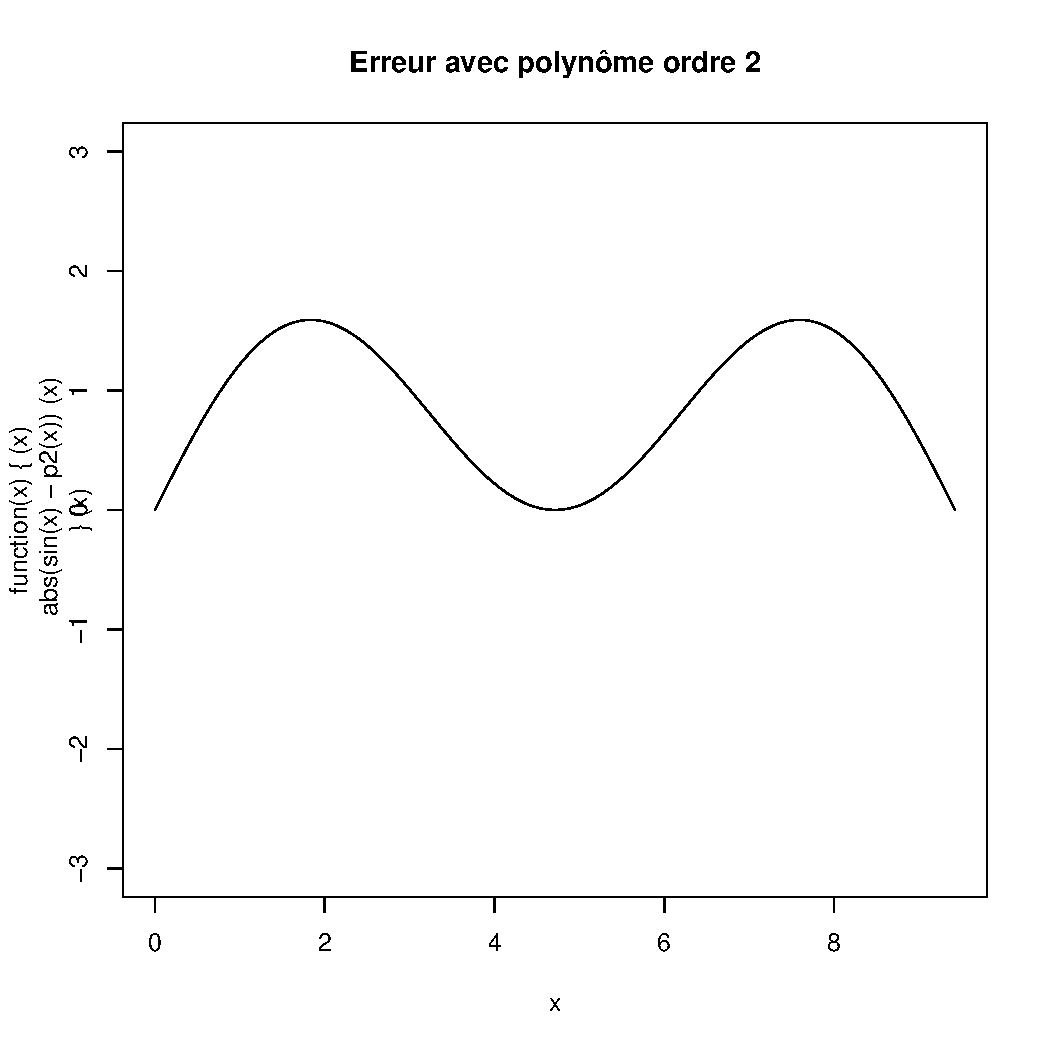
\includegraphics[scale=0.4]{data/p2}
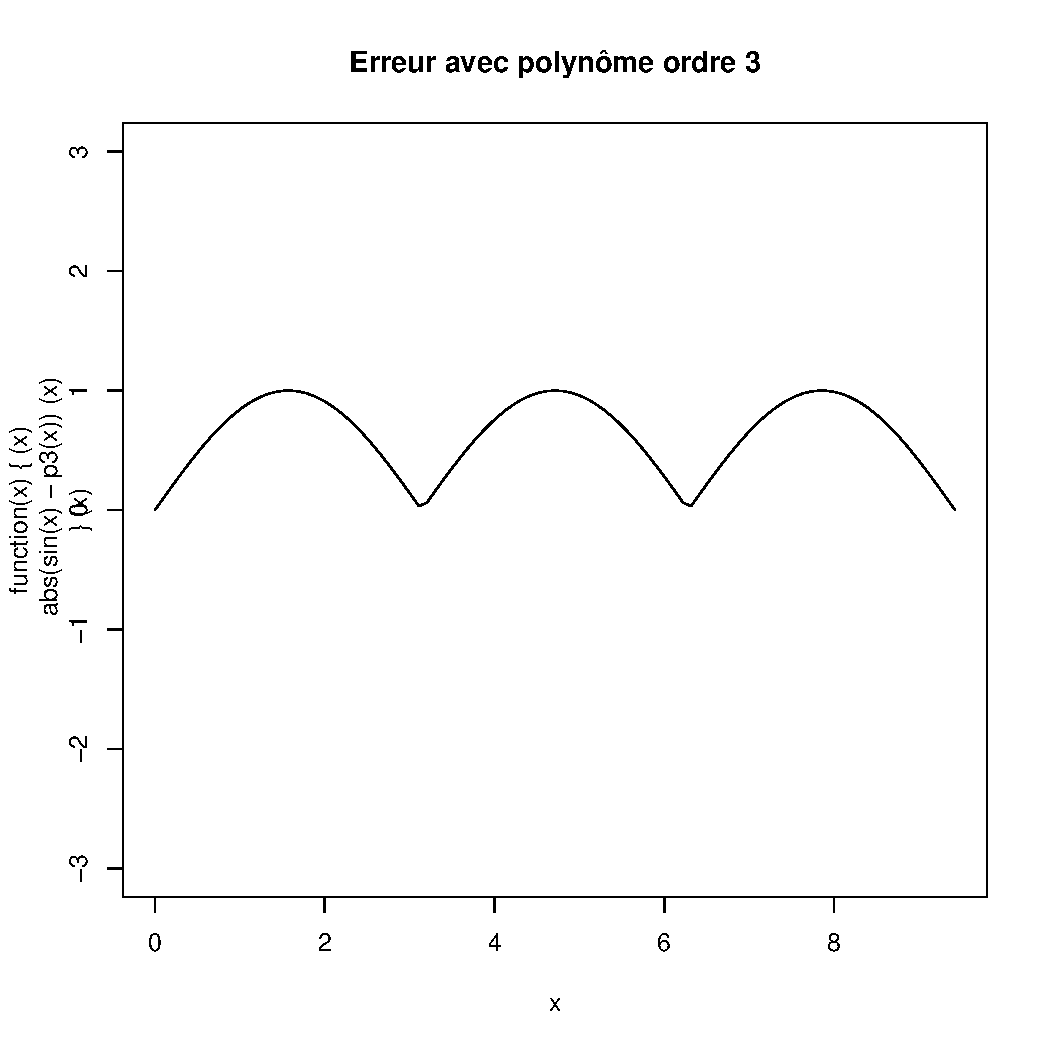
\includegraphics[scale=0.4]{data/p3}
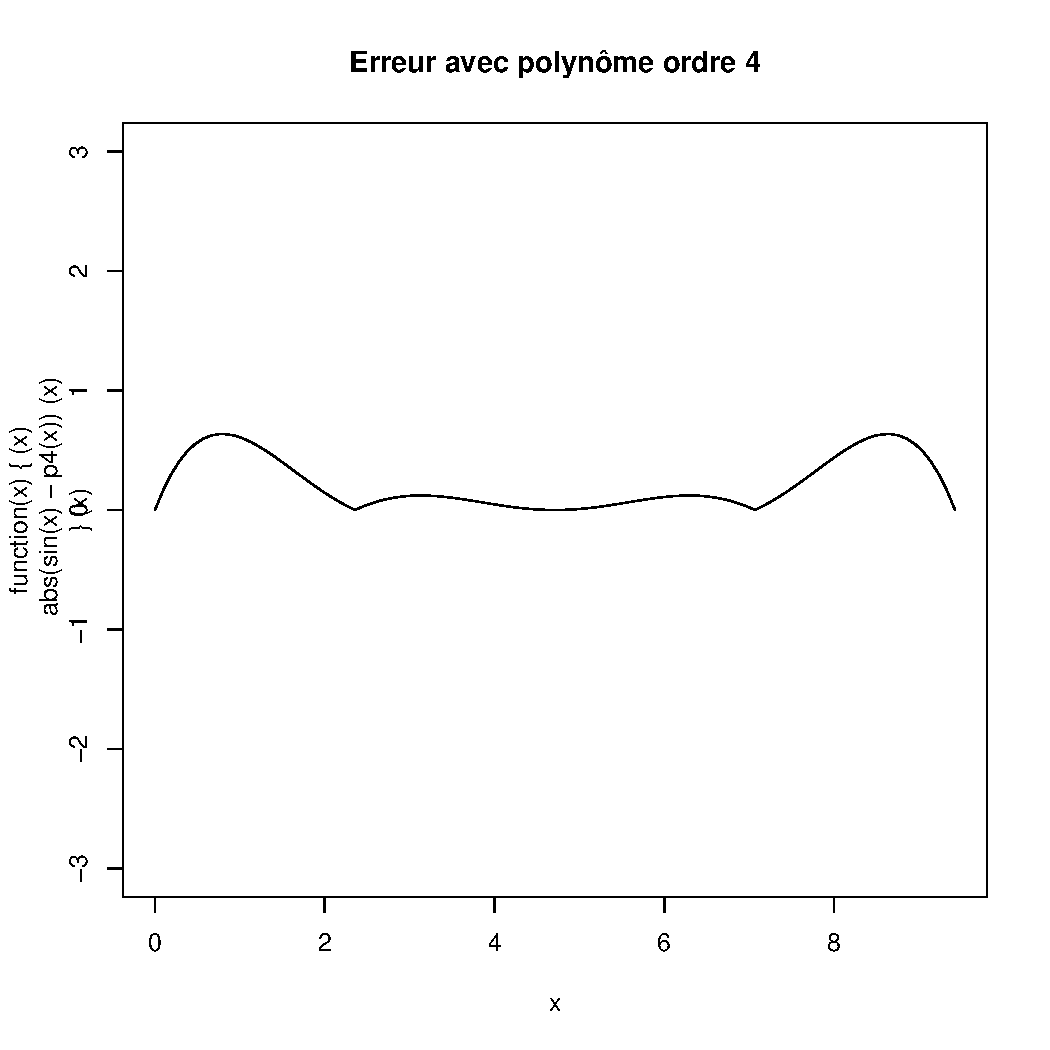
\includegraphics[scale=0.4]{data/p4}
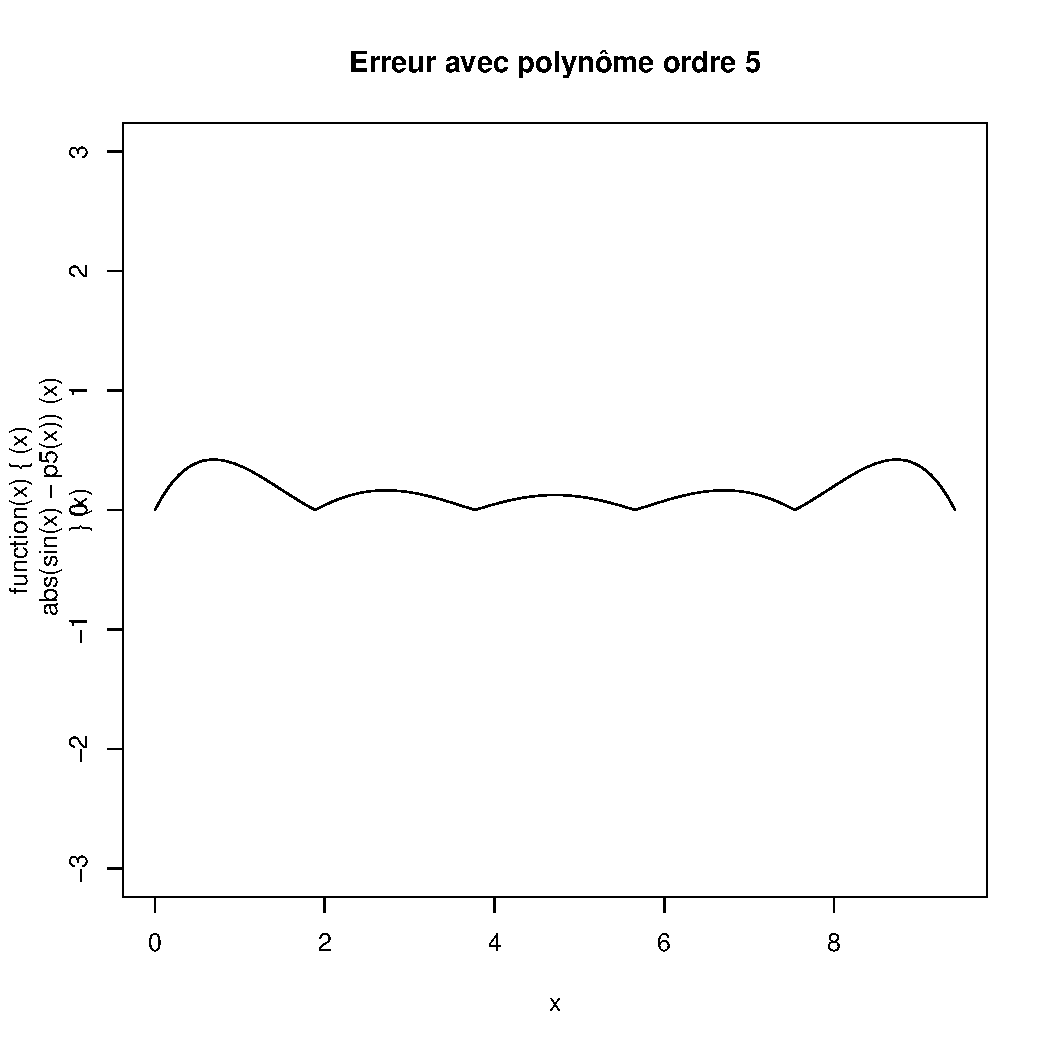
\includegraphics[scale=0.4]{data/p5}


\section{Intégration numérique}

\subsection{Description du problème et méthodes utilisées}

Le problème demande de faire la résolution numérique de l'intégrale
suivante:

\[
\int_0^1 \frac{1}{x^2 + x + 1}dx
\]

en utilisant les méthodes suivantes:

\begin{itemize}
\item Méthode des trapèzes
\item Méthode de Simpson 1/3
\item Méthode de Simpson 3/8
\end{itemize}

L'utilisateur spécifie le nombre d'intervalles à utiliser; on utilise
ce nombre directement dans la méthode des trapèzes, et pour les
méthodes de Simpson, on procède comme suit:

\begin{itemize}
\item Si le nombre d'intervalles est pair, on utilise uniquement la
  méthode de Simpson 1/3;
\item Si le nombre d'intervalles est impair, on utilise la méthode de
  Simpson 3/8 sur les 3 derniers intervalles et Simpson 1/3 sur les autres.
\end{itemize}

\subsection{Réponse aux questions}

La solution analytique de l'intégrale est $\pi/3\sqrt{3} = 0.6046$.  En
augmentant progressivement le nombre d'intervalles, les deux méthodes
(trapèzes et Simpson) convergent vers cette solution.  En examinant le
graphique ci-dessous, on peut remarquer que la méthode de Simpson
converge plus rapidement que la méthode des trapèzes.

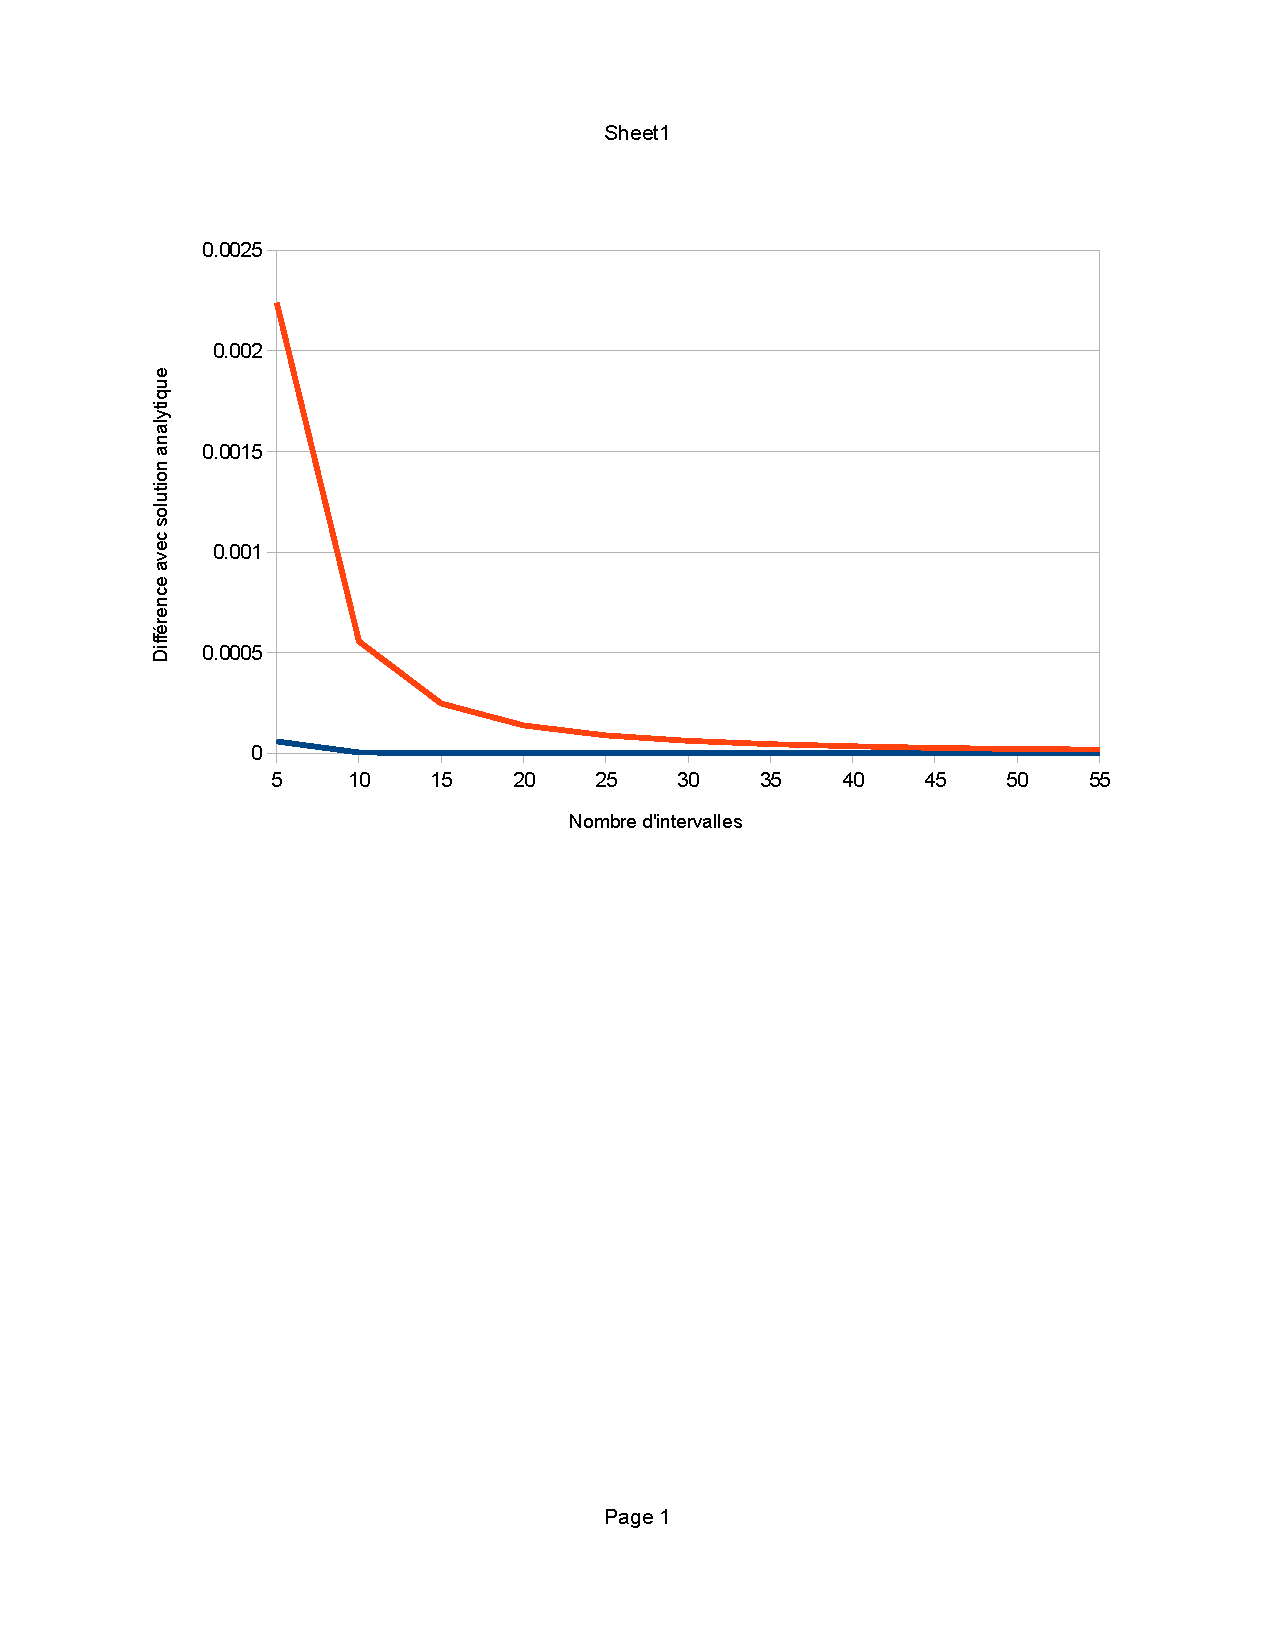
\includegraphics[scale=0.8]{delta.pdf}

\end{document}
